\documentclass[11pt,letter]{article}
\usepackage[top=0.70in, bottom=0.7in, left=1.1in, right=1.1in]{geometry}
\usepackage{graphicx} % Required for inserting images
\usepackage{xcolor} 
\definecolor{Accent}{HTML}{bd2b00} 
\usepackage[numbers,compress,super]{natbib}
\usepackage{gensymb}
\usepackage{hyperref}
\hypersetup{colorlinks,citecolor = Accent, linkcolor = Accent,urlcolor = Accent, breaklinks=true}
\usepackage{cleveref}
\usepackage[labelfont=bf]{caption}
\bibliographystyle{unsrtnat}

\RequirePackage[labelfont={bf,sf},%
                font={small, sf}]{caption}

\usepackage{lineno}
\renewcommand\linenumberfont{\normalfont\tiny\color{gray}}

\begin{document}

\title{Overlooked model uncertainties may misinform forest management strategies
% Alternative title: Integrating full model uncertainties could improve forest management
}

\author{Victor, Jérôme, Isabelle} % and more?
\date{}
\maketitle 
%emw19May -- overall this seems much better! The text is still not as tight as I would hope for a short format journal though. 

\noindent\rule{\textwidth}{0.3pt}
%emw19May -- One thing that is tricky here is the link the management. I think it's fine (and even good!) but it makes the number of links you need to make for the reader to get to your point longer. (For example, in your abstract you could just say 'Forests play a major role in mitigating climate change and maintaining that requires robust forecasts of their future composition ...' but the management connection takes more steps). Just being aware of this could help you make it as easy as possible on the reader. 
%emw19May --  alternative abstract text: 
Forests play a major role in mitigating climate change. Maintaining them requires robust forecasts to guide management. Yet, current projections are highly variable due to their reliance on layered models. Identifying sources of this variability---whether it comes from differences in either emissions scenarios, climate models or ecological models---would aid decision makers and forests managers. To this end, we compared the forecasts for European forests across 1,350 combinations of ecological models spanning a gradient from mechanistic models to correlative models as well as climate scenarios, and found that differences between ecological models were the largest source of uncertainty (40 to 64\%), surpassing differences between climate models and emission scenarios (e.g., SSP2 vs. SSP5). Despite these large uncertainties, we identified areas with relatively consistent projections where immediate management action could be taken. We also identified areas where diversified and more risk-averse strategies could be beneficial until ecological forecasting improves. Our results point to current limitations of ecological forecasting methods that hinder decision-making but also demonstrate that considering the different sources of uncertainty can improve decision-making today.

% \textbf{Abstract---still need work:} Forests play a major role in mitigating climate change, but increasing threats to forests from climate change have heightened the importance of managing these systems. Robust forecasts of forest composition with increasing climate change are critical to this aim, but are currently highly variable. To help guide management in the face of this variability and understand where we can most rapidly reduce uncertainty through improved models, we compare over 1350 ecological models and climate scenarios in forecasts for forests across Europe. Our approach considers a gradient of more mechanistic (`process-based') to correlative models of species distributions and find that difference between ecological models represent the largest source of uncertainty (40 to 64\%), surpassing both climate models and vastly different climate scenarios (e.g., SSP2 vs. SSP5). We also find areas with relatively consistent projections [give overview of these and say that this could reduce uncertainty in how to manage for these areas]. Our results point to current limitations in ecological forecasting methods, identifies avenues to lower uncertainty % vvdm: too vague?
% and, suggests that managers need to internalize ecological uncertainty through diversified and more risk-adverse strategies.

\noindent\rule{\textwidth}{0.3pt}

\linenumbers

\subsection*{Main}

Forests are key to climate change mitigation policies and achieving carbon neutrality  \citep{Korosuo2023, Hyyrynen2023}. In Europe, where summer temperatures are rising faster than anywhere on Earth \citep{CCCS2024}, some forests are already becoming net CO$_2$ sources \citep{Hadden2016, Karelin2021}. This transition is driven by unprecedented pulses of tree mortality \citep{Senf2020}, due to an increase in  burned areas \citep{Carnicer2022, Kelly2024}, and an increased frequency in pest- and drought-induced dieback \citep{Karelin2021, Cienciala2024, Latifovic2024}.

%Forest managers working to minimize current threats while also promoting long-term adaptation to climate change rely on forecasts of shifts in critical tree species. 
Minimizing these threats requires forecasts of future distribution of tree species to aid forest management under climate change. Species shifts are expected to have a major impact on timber production and on the forest economic sector \citep{Wessely2024, Hanewinkel2013}. To preserve the socio-economic functions of forests, managers need to know whether the current species will tolerate future climatic conditions, whether they can rely on natural regeneration, or whether they should consider new species opportunities. % However, to date, tree species distribution models have struggled to provide practical insights for forest management.
Despite progress in tree species distribution models, their practical relevance for forest management is still limited because models provide highly divergent projections of species distribution \citep{Morin2009, Keenan2011a, Cheaib2012, Takolander2019}.

Divergent forecasts are driven often by the underlying approach of the model, from correlative to more mechanistic. It remains unclear under which conditions one approach is more reliable than another \citep{VanderMeersch2025}, but most projections still rely on a limited set of models \citep{Dyderski2018, Wessely2024, Hanewinkel2013, Schueler2014}. This masks potentially significant uncertainties and ultimately increases the risk of supporting incorrect policy and management decisions \citep{Dawson2011}. 

Gaining a better understanding of where uncertainties originate and how they relate contributes to incorporating the current reality of uncertain forecasts into decision making \citep{Urban2016, Saltelli2020, Johnson2024, Simmonds2024}. Current projections of tree distributions compound several layers of uncertainty, climatological, biological, socioeconomic, and model-based. If most of the variation across species range shift projections is due to ecological models, even more than global emissions scenarios, it becomes critical to encompass a wide range of ecological models. Failing to do so could lead to overly confident predictions about which species will or will not be able to survive in future climates, ultimately leading to counterproductive or even detrimental forest management decisions. % and to identify policy-relevant questions ? For example, consistency between projections can reveal regions where models agree and where uncertainty is lower where management could take immediate action with low risk of failure, and identify regions where models strongly disagree for which uncertainty management and diversification of options would be necessary. 
%emw19May -- I would cut the below sentence and see if you can get by without it. 
% We must incorporate the diversity of models and merge across ecological and climatological models 

%emw19May -- below, consider integrating methods more? Something like ... (you could also add 'hybrid' term here):
To provide a complete picture of both the threats and opportunities for forests, we combined more than 1350 projections from models of forest tree species distributions from 1970 to 2100, at a 0.1\degree~spatial resolution. We incorporated a range of ecological models,  process-based, correlative and `hybrid' models. We also considered a range of climate model predictions, using 5 global climate models with different climate sensitivities, and two emissions (`forcing') scenarios, resulting in a set of 10 future climatic conditions. Projections were performed for nine species of trees, both broadleaf and needleleaf, adapted to various climatic conditions throughout Europe and representing two-thirds of Europe's forested area (Supplementary Figure 1). Including the different sources of variability in the projections allowed us to quantify the contribution of each source to the total variation between the projections. 
% This approach represents a significant advancement over previous studies, which overlooked large portions of uncertainty. Such advances could lead to more informed decision-making to improve the resilience of forests. 

\begin{figure}
	\centering
	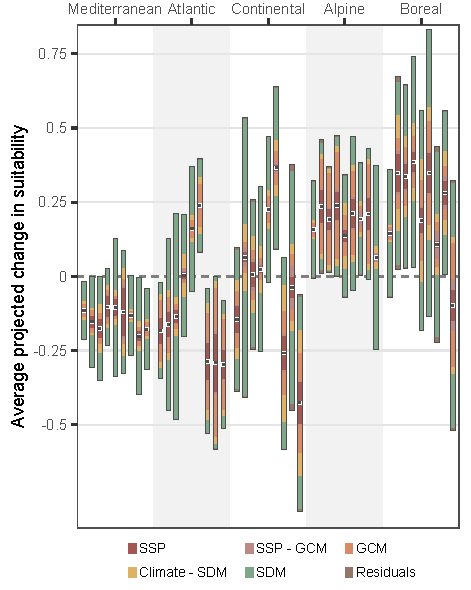
\includegraphics[width=1\linewidth]{figures/anova_within_species_byecoregion-1.pdf}
	\caption{\textbf{Ecological models represent the main source of uncertainty in future projections of species climatic suitability across European biomes (2080-2100).} Level of uncertainty associated with projected changes in suitability relative to the historical period (1970–2000), \textbf{(a)} for each species within biome and \textbf{(b)} across all species and biomes. The five main European biomes are represented in \textbf{(c)}. Five uncertainty sources are distinguished: (i) the future scenario (SSP), (ii) the climate model used to generate the climate projections (GCM), (iii) the interactions between the SPP and the GCM, (iv) the species distribution modeling method (SDM), and (v) the interactions between SDM and climate projections (both GCMs and SSPs). For each species, the black line represents the mean projection, across all GCMs, SSPs, and SDMs. 90\% uncertainty ranges were calculated additively and symmetrically around the mean.}
	\label{fig:anovaspecies}  %emw19May -- what is (c)? Add to caption.
\end{figure}

\subsection*{Results and discussion}

Differences between ecological models consistently explained more variation than vastly different climate trajectories. We found that the choice of the ecological model explained 51\% of the uncertainty in species range shift across species and biomes, while the choice in the socio-economic pathway explained 35\% of the uncertainty (\Cref{fig:anovaspecies}). In the driest biome, the Mediterranean region, a consistent decline in suitability was observed for all species. The Atlantic and Continental biomes showed conflicting and generally non-significant trends, making conclusions difficult (\Cref{fig:anovaspecies}). The example of sessile oak in the Atlantic region, where this species represents an important cultural and economic value, illustrates this clearly: more than 80\% of the uncertainty in the projections is due to variations among the ecological models. 

% The differences among climate model projections (GCMs) and socioeconomic scenarios (SSPs). 
% in the Continental ecoregion, differences across models account for 73.7% of the total uncertainty of beech future suitability, despite being within the core of its present distribution. Similarly, SDM is the main source of uncertainty for sessile and pedunculate oaks (respectively 57% and 76.8%, Figure 22).

\subsubsection*{Mechanistic to correlative models contribute to high uncertainty...}

Accounting for more diverse ecological models led to a wider range of predicted changes in suitability. \Cref{fig:cascade} shows that---on average across all species---correlative models alone offer a restricted view, whereas much of the variability arises at the ecological level (models and their parameters). This strong divergence between ecological models reveals the persistent gaps in our understanding of species responses to climate change. Considering only correlative models would have led to an overestimation of the contribution of climate projections (forcing scenarios, climate models, and their two-way interaction) to the total projection uncertainty in all regions, except the Mediterranean. In particular, divergence between climate models would have appeared to contribute as much as ecological models to projection uncertainty (on average, 36.6\% and 37.5\%, respectively, Supplementary Figure 2). 

\begin{figure}
	\centering
	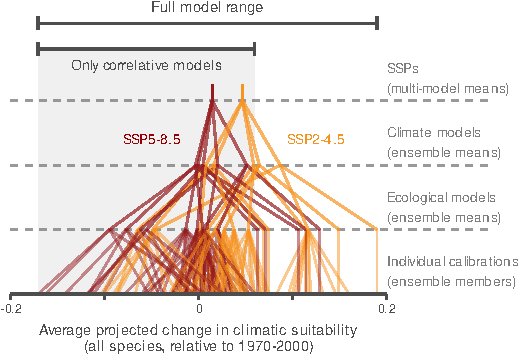
\includegraphics[width=0.75\linewidth]{figures/allspecies_cascade.pdf}
	\caption{\textbf{Considering a broad range of models provides a more comprehensive view of possible futures .} This figure illustrates the average change in suitability across all species and all biomes, with the hierarchical contribution of each source of uncertainty. The top of each cascade represents the overall average change in suitability for each Shared Socioeconomic Pathway (SSP). The level below shows the ensemble mean for each climate model (5 branches per SSP, corresponding to the 5 GCMs considered here), averaged across multiple ecological models. The next level represents the contribution of each ecological modeling approach (mechanistic, hybrid, and correlative, 3 branches per GCM). The final level displays the variations within each approach (e.g., different parameter calibrations or statistical algorithms), although for mechanistic models only a single calibration was available. This figure was inspired by the Figure 1.15 in IPCC, 2021: Chapter 1.}
	\label{fig:cascade}
\end{figure}

Using a comprehensive set of models, from correlative to mechanistic, avoids the specific biases inherent in some modeling approaches. Our results revealed that models calibrated using current species range data (correlative and hybrid) consistently predict greater extinction risks than mechanistic models calibrated using experimental data (\Cref{fig:diffproj}). 
Current distribution data may capture only a portion of the climatic niche of a species, underestimating the range of conditions where it could survive \citep{Chevalier2024, NoguesBravo2016}.

These discrepancies between models can significantly alter country-level projections and impact national strategies derived from them. 
Beech provides a case example. By the end of the 21st century, beech is predicted to decrease in  suitability of -0.19 ($\pm$0.14, Supplementary Table 1) in its historical distribution based on species distribution models calibrated with current species distribution data, leading to an average loss of 30.5\% of its distribution (\Cref{fig:diffproj}). However, a broader range of models results in a different conclusion, that is a lower net loss in beech's area (-0.028 $\pm$0.17).
Relying on a narrow set of models % , especially derived from the same calibration process, 
provides an incomplete picture \citep{Dawson2011} and can bias decisions towards intensive intervention strategies, such as the introduction of species outside of their native range.
% Multi-model ensembles have been so far mostly restricted to statistical models (Simmonds et al, 2024), but we show here that there is a strong interest in considering a broader range of models to better characterize projections uncertainty. 

\begin{figure}
	\centering
	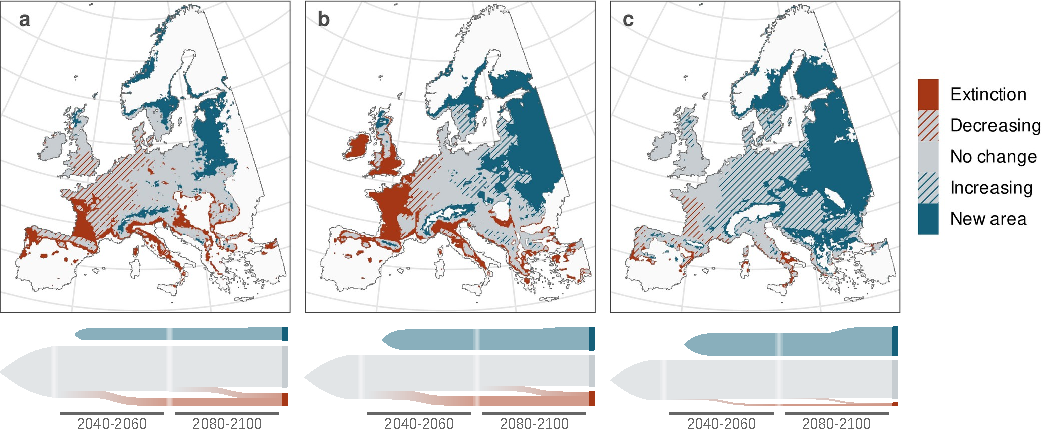
\includegraphics[width=1\linewidth]{figures/fagus_sankey.pdf}
	\caption{\textbf{Models build on current species range data project higher extinctions.} This figure illustrates the average projection of beech distribution under scenario SSP2-4.5, for each of the 3 ecological modeling approaches considered here: \textbf{(a)} correlative, \textbf{(b)} hybrid and \textbf{(c)} mechanistic models. The upper maps show the projected change in beech distribution for 2080–2100, relative to its historical distribution (1970-2000). The lower Sankey diagrams illustrate the temporal dynamics of beech distribution, from its historical distributions to projected distributions for 2040–2060 and 2080–2100. At each time interval, the width of the flows is proportional to the spatial extent where the species has gone extinct, persists, or could expend. }
	\label{fig:diffproj}
\end{figure}

\subsubsection*{Forest management strategies in an uncertain world}

Our ensemble of model results sheds light on areas with relatively consistent projections and, therefore, where actions for adaptation could be decided with higher confidence (\Cref{fig:manag}). For example, around the Mediterranean Basin, models consistently predicted less favorable climatic conditions for all species considered. In areas where most species are threatened, forest managers may thus consider introducing more heat- and drought-tolerant species. Along the Atlantic margin, the suitability of most species is also projected to decrease, except for the two Mediterranean species---pubescent and evergreen oaks--- which may naturally replace less adapted temperate species such as beech \citep{Penuelas2003}. Mechanistic model projections are less pessimistic for deciduous oaks and beech (\Cref{fig:diffproj}), suggesting that these species might cope with climate change if managers adopt certain adaptive management actions. For example, decreasing stand density to limit competition for water could support their long-term survival to drought events \citep{Young2023}. Additionally, if the existing standing genetic variation is maintained and promoted by forest managers, better-adapted genetic material could survive and be used in genetic enrichment plans \citep{Brang2014}. Finally, climatic suitability was projected to increase in boreal biomes in Scandinavian and Baltic countries (\Cref{fig:manag}). These include Finland and Sweden, two very important forest countries in terms of wood stock, added value, and forest-based workforce [CITE]. Forests in these regions are dominated by two conifer species, Scots pine and Norway spruce, which have been favoured for decades for commercial reasons. Insufficient experimental data prevented us from making mechanistic model projections for spruce, but uncertainty for Scots pine future suitability was very high. Models consistently project that temperate deciduous trees will become more competitive at the northern margin of their range (\Cref{fig:diffproj}), and extending growing seasons could offer an opportunity to convert pure coniferous stands into mixed forest to increase their resilience \citep{Schauer2023}.

Our framework also identified regions of high uncertainty, highlighting where diversification strategies are most required.
A large part of the Continental biome exhibits less clear trends (\Cref{fig:manag}), as well as mountainous regions at the transition between Mediterranean and Continental/Atlantic climates (Pyrenees, Massif Central, Balkans). A key lever of management action in this region would thus be the diversification of tree species, as well as increasing genetic diversity within populations, to mitigate the risks associated with uncertain future conditions \citep{Morin2014, Ammer2019, Pretzsch2021, Vospernik2024}. Promoting uneven-aged stands could also enhance forest stability by improving structural complexity and buffering against climate extremes \citep{Vangi2024, Zhang2024a}.

Even in these highly uncertain regions our results still highlight some smaller zones of consistency. Models agree on a lower suitability for Scots pines (with uncertainty driven more by climatic models and scenarios, 45.7\%, than by ecological models, 30.8\%), which is the dominant species in more than 30\% of forests (Supplementary Figure 1) and a commercially very important species in several countries of Central Europe [cite]. %(such as Poland, Eastern Germany, Czech Republic, Belarus).
Projections also suggest that temperate deciduous species (e.g. beech, deciduous oaks) will be less affected by climate change, despite high uncertainties due to high divergence among ecological models that account for 45.7 and 75.4\% of the total uncertainty respectively. Together, these findings contribute to a more complete view of both the threats and opportunities facing forests in Europe, and highlight regions where policies have to be carefully tailored to effectively address all uncertainties.


% supp idea: Forest management decisions can only be made alongside the development of economic sectors for deciduous species

\begin{figure}
	\centering
	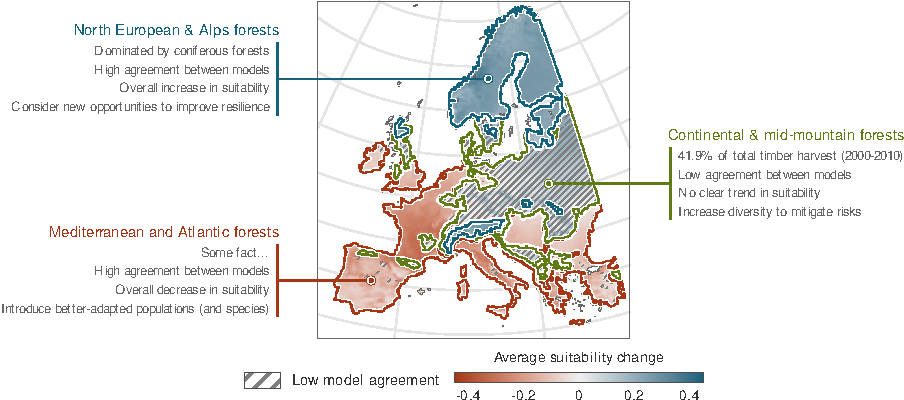
\includegraphics[width=1\linewidth]{figures/suit3-1.pdf}
	\caption{\textbf{Accounting for uncertainties supports evidence-based forest management.} Our framework allows to identify 3 areas that differ in terms of uncertainty levels, future climate risks and levers of action to address them. The map shows the average suitability change across all climate models, all ecological models and all species. Dashed areas highlight regions where the three types of ecological models (mechanistic, hybrid and correlative) do not agree on the sign of suitability change.}
	\label{fig:manag}
\end{figure}
% conifer-dominated forestry

\subsubsection*{Advancing on two fronts: move forward with uncertainty while aiming to reduce it by improving ecological models}

The large uncertainties we found clearly raise questions about the robustness of existing projections and highlight that further advances are necessary to provide the most useful projections for managers and policy makers. 
% Manque une sorte de phrase de transition.?
Correlative models are becoming more mechanistic by integrating experimental data \citep{Wagner2023}---yet, with some caution \citep{Chevalier2024a}. Combining deep learning with process-based models offers a promising approach to improve climate predictions \citep{Kochkov2024}, with a lower computational cost that could facilitate a more comprehensive estimation of uncertainties. These breakthroughs are enhancing our ability to obtain more robust ecological and climatological forecasts, and could in turn reveal new adaptive pathways for forest management. However, these improvements should not prevent us from providing a better framework to identify uncertainty in projections that can guide management, such as the framework we present here.  

The implications of our results extend beyond European forests. Mechanistic models have also been developed for North America and Asia \citep{Morin2007, Fang2022}. Their projections could be systematically integrated in a comprehensive framework such as ours, alongside correlative model projections. Such continental-scale uncertainty assessment---going beyond regional analyses \citep{Iverson2016}---would provide more robust guidance for forest management. This is particularly critical in countries where forests are managed at a broader scale than in Europe---such as the United States---and where it could thus be easier to incorporate uncertainty into large-scale decision making. 

Given the rapid pace of climate change, rather than debating over which modeling approach to favor, efforts should focus on bridging diverse methodologies to generate practical insights and support evidence-based decision making. Ultimately, as scientists, we need to be transparent about projection uncertainties if we expect forest managers to acknowledge and integrate them \citep{Saltelli2020}. This is how ecological modeling can become truly relevant to decision making in the context of climate change.


\subsection*{Methods}

\subsubsection*{Species distribution models}

We sought to encompass a broad diversity of species distribution models by including three different approaches: correlative models, mechanistic models and hybrid models (i.e. mechastic models calibrated like correlative models\citep{VanderMeersch2023}).

For the correlative approach, we selected four well-established models\citep{Valavi2022}: GLM with lasso regularization, GAM, BRT, and down-sampled Random Forest. For the mechanistic approach, we used the process-based model PHENOFIT. The model has been validated for several North American and European species, either in historical or Holocene climatic conditions \citep{Morin2007, Saltre2013, Duputie2015, Gauzere2020, VanderMeersch2025}. For the hybrid approach, we calibrated PHENOFIT using the same species occurrence data as correlative models\citep{VanderMeersch2023}. We optimized the parameters of the model using the covariance matrix adaptation evolution strategy\citep{Hansen2001}.

\subsubsection*{Climate projections}

Future simulations were run with the last Coupled Model Intercomparison Project Phase 6 (CMIP6) climate  projections, for 5 global climate models (GCMs) and 2 shared socio-economic pathways (SSPs). 
We used model projections that were downscaled to a 0.1° resolution with a statistical trend-preserving method (the cumulative distribution function transform), using the ERA5-Land reanalysis as a reference observational dataset between 1981 and 2010 \citep{Noel2022}. We used the projections of five GCMs considered as good representatives of the full CMIP6 ensemble \citep{Noel2022} : GFDL-ESM4 \citep{Dunne2020}, IPSL-CM6A-LR \citep{Lurton2020}, MPI-ESM1-2-HR \citep{Mueller2018}, MRI-ESM2-0 \citep{Yukimoto2019} and UKESM1-0-LL \citep{Sellar2020}.  

\subsubsection*{Uncertainty partitioning}

Our approach was inspired by the partitioning of uncertainties in climate projections initially developed by Hawkins and Sutton \citep{Hawkins2009, Hawkins2011}, which was subsequently enhanced with additional methodologies \citep{Yip2011, Lafferty2023}. Rather than using a simple variance decomposition approach, we perform an ANOVA-based variance decomposition to also estimate the importance of the two-way interaction effects. All analyses were performed in R \citep{RCT2024}.

Across all species, we partitioned three sources of uncertainty: the climate projection uncertainty related to the different GCMs, SSPs, and their interaction, the species distribution modeling uncertainty related to the differents SDMs. We also considered the interactions between SDMs and climate projections (GCMs and SSPs). For each year, the suitability of a cell was considered as a 21-year moving average suitability (e.g. 2040-2060 for the year 2050). We then computed the difference of suitability with the historical suitability (c1970-2000). For each GCM and each SSP, when multiple SDM projections were simulated within the same SDM approach (e.g. multiple algorithms for correlative approach), we kept one ensemble per approach. For each year $t$, we then applied a linear ANOVA to calculate the sums of squares attributable to each uncertainty source:
$$
{SS}_{tot} = {SS}_{GCM} + {SS}_{SSP} + {SS}_{GCM:SSP} + {SS}_{SDM} + {SS}_{SDM:GCM} + {SS}_{SDM:SSP} + {SS}_{residuals}
$$

We then computed 90\% uncertainty ranges additively and symmetrically around the mean projection (across all GCMs, SSPs, SDMs), e.g. for SDM uncertainty: $\pm1.645*\sigma*\frac{{SS}_{SDM}}{{SS}_{tot}}$.


\clearpage

\bibliography{phd_bibliography}

\end{document}
